\section{Solution r\'ealis\'ee}

\begin{frame}
 	\frametitle{Solution r\'ealis\'ee}
        \tableofcontents[currentsection,hideothersubsections]
\end{frame}

\subsection{Fonctionnalit\'es impl\'ement\'ees}
\frame
{
\frametitle{Fonctionnalit\'es impl\'ement\'ees}
\framesubtitle{Fonctionnalit\'es du programme final}
\begin{itemize}
 \item<1-8> R\'ecup\'eration d'informations sur un AS
 \item<2-8> Calcul du nombre de cliques maximum dans le graphe gr\^ace \`a l'algorithme de Bron and Kerbosch
 \item<3-8> Chargement d'un fichier de triplets pour \'eliminer les stubs du graphe
 \item<4-8> Zoomer sur le proche voisinage d'un AS
 \item<5-8> Revenir au graphe de base
 \item<6-8> Calculer la centralit\'e de Freeman des sommets
 \item<7-8> Filtrer les sommets selon leur centralit\'e
 \item<8> Filtrer les sommets selon leur num\'ero d'AS
\end{itemize}
}
\frame
{
\frametitle{Fonctionnalit\'es impl\'ement\'ees}
\framesubtitle{S\'equence des options}
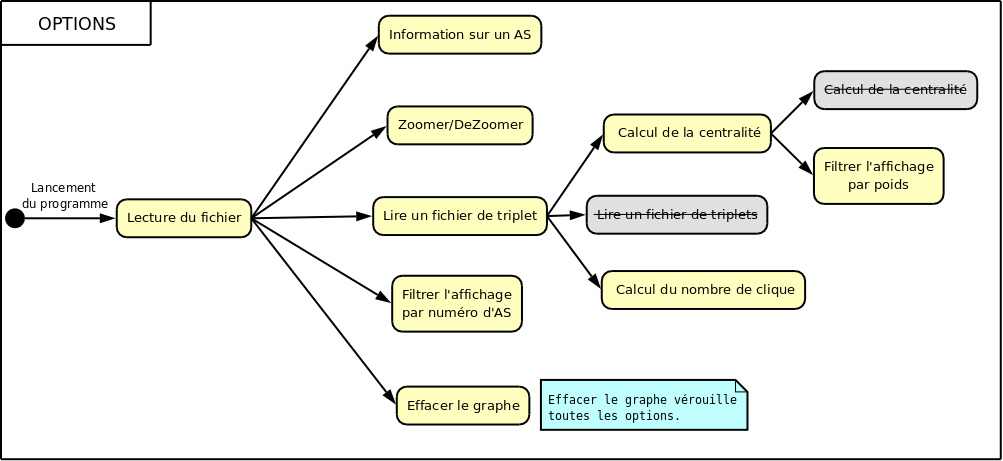
\includegraphics[width=\textwidth]{./seqMenu.png}
}

\subsection{Rendu final}
\frame
{
\frametitle{Rendu final}
\only<1>
{
   \begin{center}
   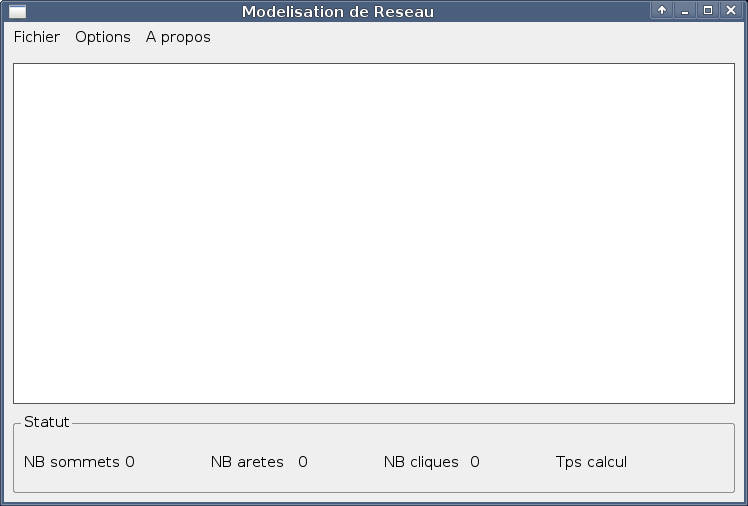
\includegraphics[width=0.9\textwidth]{ecran_programme.png}\\
   Ecran principal du programme
   \end{center}
}
\only<2>
{
   \begin{center}
   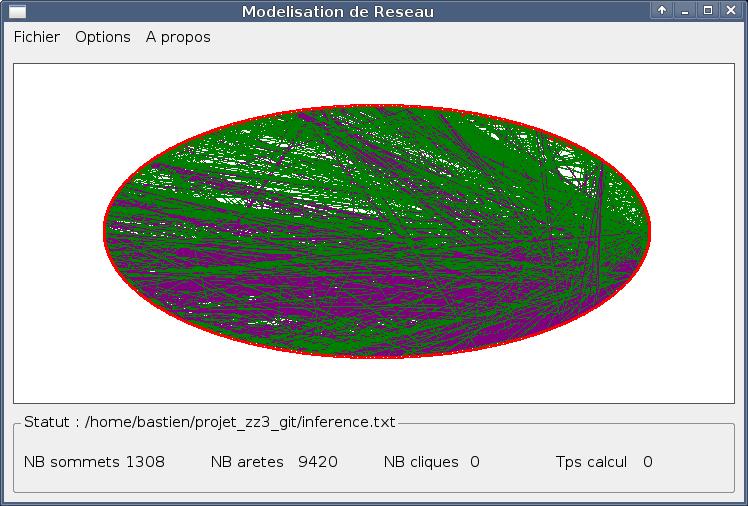
\includegraphics[width=0.9\textwidth]{ecran_graphe.png}\\
   Graphe charg\'e
   \end{center}
}
\only<5>
{
   \begin{center}
   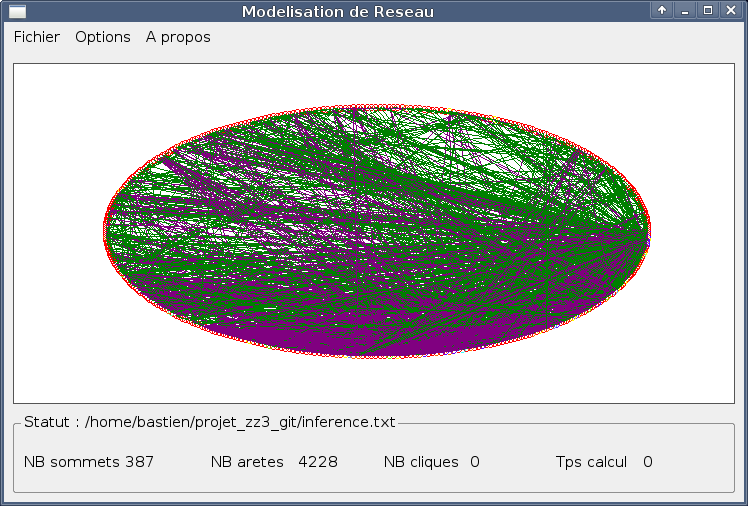
\includegraphics[width=0.9\textwidth]{ecran_graphe_nostubs.png}\\
   Stubs \'elimin\'es
   \end{center}
}
\only<6>
{
   \begin{center}
   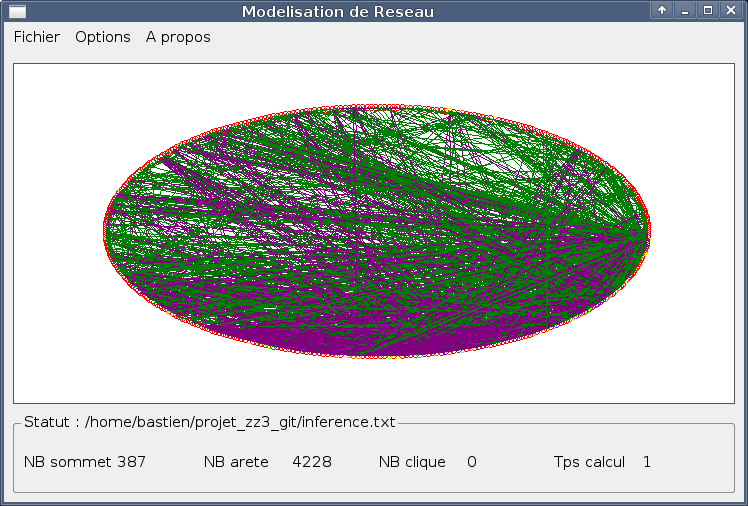
\includegraphics[width=0.9\textwidth]{ecran_graphe_centrality.png}\\
   Centralit\'e calcul\'ee
   \end{center}
}
\only<3>
{
   \begin{center}
   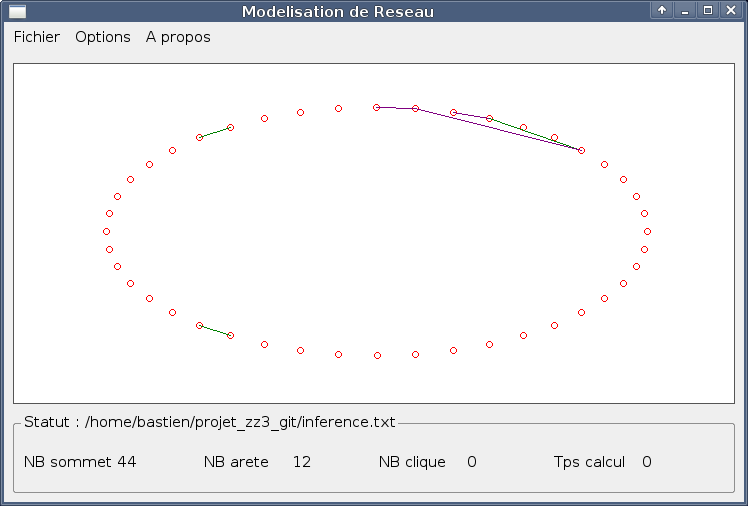
\includegraphics[width=0.9\textwidth]{ecran_graphe_filtre.png}\\
   Filtrage par num\'ero d'AS
   \end{center}
}
\only<4>
{
   \begin{center}
   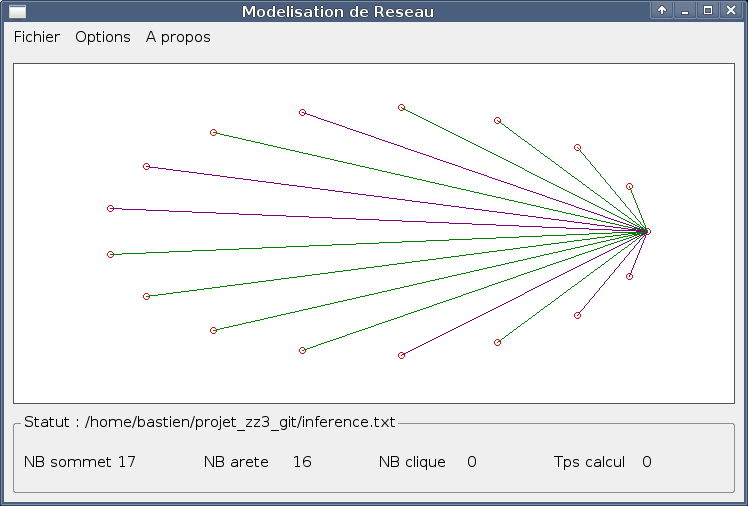
\includegraphics[width=0.9\textwidth]{ecran_graphe_zoom.png}\\
   Zoom sur un AS
   \end{center}
}
}